\documentclass[norsk,a4paper,12pt]{article}
\usepackage[T1]{fontenc} %for å bruke æøå
\usepackage[utf8]{inputenc}
\usepackage{graphicx} %for å inkludere grafikk
\usepackage{verbatim} %for å inkludere filer med tegn LaTeX ikke liker
\usepackage{mathpazo}
\usepackage{listings}
\bibliographystyle{plain}
\usepackage{xcolor}
\usepackage{float}
\usepackage{amsmath}

\setlength{\parindent}{0em}

\definecolor{background}{gray}{0.9}
\definecolor{comment}{rgb}{0.6,0.4,0.8}
\definecolor{string}{rgb}{0.6,0.4,0.8}
\definecolor{keyword}{rgb}{0.9,0.17,0.31}
\lstset{
	title=\lstname,
	numberstyle=\tiny, 
	breaklines=true,
	tabsize=4,
	language=Python,
	morekeywords={with,super,as},,
	frame=single,
	basicstyle=\footnotesize\tt,
	commentstyle=\color{comment},
	keywordstyle=\color{keyword},
	stringstyle=\color{string},
	backgroundcolor=\color{background},
	showstringspaces=false,
	numbers=none,
	numbersep=5pt,
	literate=
		{æ}{{\ae}}1
		{å}{{\aa}}1
		{ø}{{\o}}1
		{Æ}{{\AE}}1
		{Å}{{\AA}}1
		{Ø}{{\O}}1
	}


\title{Prosjektoppgave besvarelse}
\author{Kadnidatnummer: 15267}
\date{\today}
\begin{document}

\maketitle


\section*{Oppgave 1}

Ved å løse differensial likningen
\\

\begin{equation}
	m\ddot{x}(t) + kx(t) =0,
\end{equation}

og plotte systemets bane i faserommet så får vi plottet i figur \ref{fig:plotoppg1}
\\
\begin{figure}[H]
\begin{center}
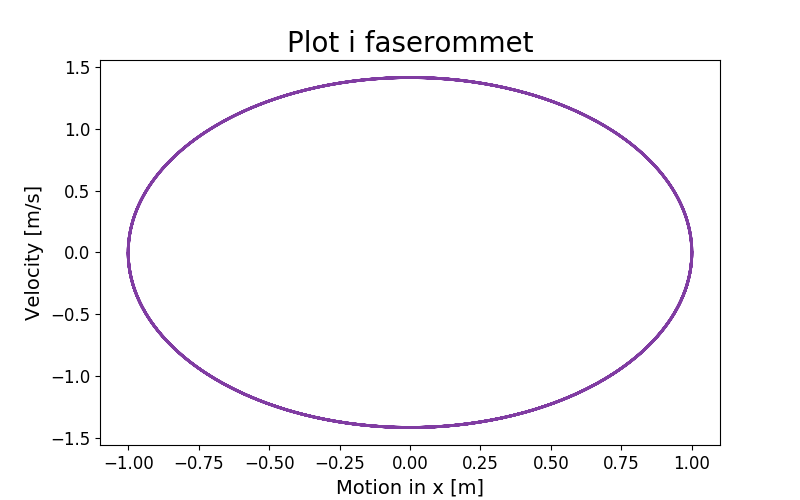
\includegraphics[scale=0.5]{Oppgave1fase.png}
\caption{viser faseplottet for en fri harmonisk oscillator}
\label{fig:plotoppg1}
\end{center}
\end{figure}

Hvis vi varier initialverdiene for posisjonen og hastigheten, så vil det fortsatt være en ellipse. Hvis vi ser på totalenergien til systemet så ser vi hvorfor dette stemmer. Totalenergien er 

\begin{align*}
	E_{tot} =& E_k + E_p\\
	E_{tot} =& \frac{1}{2}m\dot{x}^2 + \frac{1}{2}kx^2\\
	\frac{2E_{tot}}{mk} =& \frac{\dot{x}^2}{k} + \frac{x^2}{m},\\
	Hvis\ vi\ setter\ C =& \frac{2E_{tot}}{mk}\\
	\Rightarrow \frac{x^2}{m} + \frac{\dot{x}^2}{k} =& C \\
	\frac{x^2}{mC} + \frac{\dot{x}^2}{kC} =& C \\
	\frac{x^2}{\sqrt{mC}^2} + \frac{\dot{x}^2}{\sqrt{kC}^2} =& 1 \\
\end{align*}

Det er formelen for en ellipse.
\\
\\
Der hvor banen krysser x aksen og y aksen så er den vinkelrett på den aksen den krysser. Dette skyldes at i de punktene så er totalenergien lokalisert i bare det ene uttrykket, og det andre er null. Ved $|x| = max$ så endrer bevegelsen retning og $E_{tot} = E_p$. Når $x=0$ så er $E_{tot}=E_k$
\\
\\
Hvis vi plotter en kortere tidsperiode slik at kurven ikke når til startposisjonen så ser vi at den beveger seg med klokken. Selv om vi varierer startposisjon og starthastighet så er det ikke mulig å få banen til å gå i motsatt retning på grunn av hvordan vi har satt positive retninger og hva vi har satt på x og y aksen.
\\




\section*{Oppgave 2}
Hvis vi inkluderer dempning i programmet så vil banen i faseplottet gå gradvis mot punktet $x = 0m$ og $\dot{x} = 0 m/s$ som en spiral.
\\
\\
\begin{figure}[H]
\begin{center}
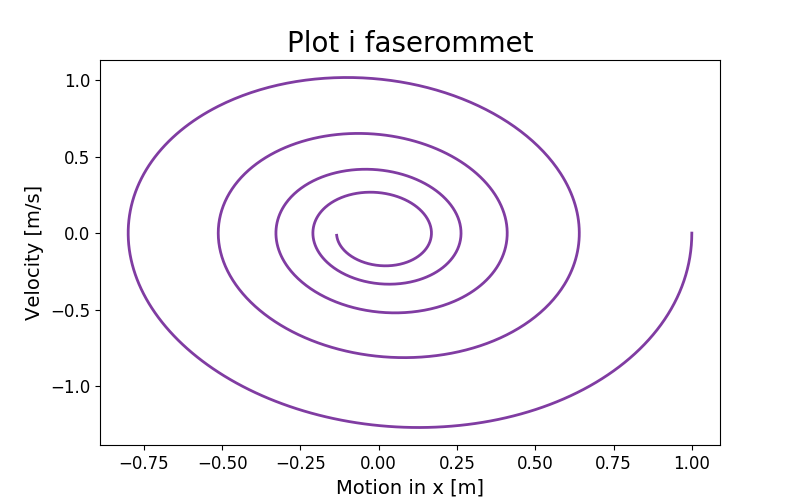
\includegraphics[scale=0.5]{Oppgave2fase.png}
\caption{viser faseplott for svingning med dempning}
\label{fig:faseplot2}
\end{center}
\end{figure}

Banen står vinkelrett bare når den krysser x aksen, ikke y aksen. Dette er på grunn av dempings leddet som vi satt inn. 
\\
\\
En attraktor er et set med numeriske verdier som et dynamisk system har en tendens til å utvikle seg mot for et bredt utvalg av initialbetingelser. En attraktor kan være et punkt(0 dim), et set met punkter, en kurve(2 dim), og flere ting innenfor matematikk. Punktet $x=0m$ og $\dot{x}=0m/s$ er en attraktor av dimensjon 0, fordi det er et singulært punkt. Kurven i oppgave 1 er også en attraktor i følge definisjonen, siden systemet alltid havner i den kurven uansett initialbetingelser og er av dimensjon 1. 





\section*{Oppgave 3}

Vi skal løse følgende likning alanytisk.
\\
\\
\begin{equation}
	m \ddot{x}(t) +kx(t) = F_D cos(\omega_Dt)
	\label{eq:diffpatrykt}
\end{equation}

Begynner med å finne den generelle løsningen for den homogene likningen, og løser derfor den karakteristiske likningen $m\lambda^2 + k = 0$

\begin{align*}
	m\lambda^2 + k =& 0 \\
	\lambda^2 =& \frac{-k}{m} \\
	\lambda =& \pm \sqrt{\frac{-k}{m}}\\
\end{align*}

Hvis vi har $\lambda$ på formen $\lambda_{\pm} = \mu \pm i\eta$, så får vi den generelle løsningen

\begin{align*}
	\lambda =& \pm i \sqrt{\frac{k}{m}}\\
	x_h =& e^{\mu t}(A cos(\eta t) + B sin(\eta t))\\
	x_h =& e^{0t} \left(A cos \left(\sqrt{\frac{k}{m}}t\right) +B sin \left(\sqrt{\frac{k}{m}}t \right) \right)\\
	x_h =& \underline{A cos \left(\sqrt{\frac{k}{m}}t \right) +B sin \left(\sqrt{\frac{k}{m}}t \right)}\\
\end{align*}

Så den generelle løsningen for den homogene delen er

\begin{equation}
	x_h = A cos \left(\sqrt{\frac{k}{m}}t \right) +B sin \left(\sqrt{\frac{k}{m}}t \right)
\end{equation}


Nå skal vi bruke metoden for ubestemte koeffisienter for å finne den partikulære løsningen. Siden høyre side av likningen er på formen $A cos(pt)$, så kan vi bruke $x_p$ på formen $C e^{ipt}$

\begin{align*}
	x_p =& C e^{ipt},\   \   \ p=\omega_D, fra\ \ likningen\\
	x_p =& C e^{i\omega_Dt}\\
	\dot{x_p} =& iC\omega_D e^{i\omega_Dt}\\
	\ddot{x_p} =& -C\omega_D^2 e^{i\omega_Dt}\\
\end{align*}

Dette setter vi inn i difflikningen og løser for C

\begin{align*}
	m\ddot{x} + kx = F_D cos(\omega_Dt)\\
	m\left(-C\omega_D^2e^{i\omega_Dt} \right) + k Ce^{i\omega_Dt} =& F_Dcos(\omega_Dt)\\
	-mC\omega_D^2e^{i\omega_Dt} + k Ce^{i\omega_Dt} =& F_Dcos(\omega_Dt)\\
	Ce^{i\omega_Dt} \left(-m\omega_D^2 +k \right) =& F_Dcos(\omega_Dt)\\
	C =& \frac{F_Dcos(\omega_Dt)}{e^{i\omega_Dt} \left(-m\omega_D^2 +k \right)}\\
\end{align*}

Så setter vi uttrykket for C inn i $x_p$ og får at

\begin{equation}
	x_p = \frac{F_Dcos(\omega_Dt)\\}{\left(k - m \omega_D^2 \right)}
\end{equation}

Så den fullstendige generelle løsningen er

\begin{equation}
	A cos \left(\sqrt{\frac{k}{m}}t \right) +B sin \left(\sqrt{\frac{k}{m}}t \right) + \frac{F_Dcos(\omega_Dt)\\}{\left(k - m \omega_D^2 \right)}
\end{equation}

Vi skulle løse den for $x(0)=2m$ og $\dot{x}(0)=0 m/s$, så da gjør vi det og får 

\begin{align*}
	A =& 2 - \frac{F_D}{k-m\omega_D^2}\\
	B =& 0\\ 
\end{align*}

Dette setter vi inn i løsningen og får

\begin{equation}
	x(t) = 2 cos \left(\sqrt{\frac{k}{m}}t \right) + \frac{F_D}{k-m\omega_D^2} \left(cos(\omega_Dt)-cos \left(\sqrt{\frac{k}{m}}t \right) \right)
\end{equation}

Så bruker vi en trigonometrisk identitet funnet på side 42 i Rottmann, som ser slik ut

\begin{equation}
	cos \alpha - cos \beta = -2 sin\frac{\alpha + \beta}{2}sin\frac{\alpha -\beta}{2}
\end{equation}

og da får vi

\begin{equation}
	x(t) = 2 cos \left(\sqrt{\frac{k}{m}}t \right) - \frac{2F_D}{k-m\omega_D^2} \left(sin\frac{\left(\omega_D + \sqrt{\frac{k}{m}} \right)t}{2} sin\frac{\left(\omega_D - \sqrt{\frac{k}{m}} \right)t}{2} \right)
\end{equation}

Siden uttrykket består av cosinus og sinus så vet vi at den er periodisk på et eller annet vis.
\\
\\

\section*{Oppgave 4}
Ved å løse likning \ref{eq:diffpatrykt} nummerisk og plotte den nummeriske løsningen minus den analytiske så får vi.

\begin{figure}[H]
\begin{center}
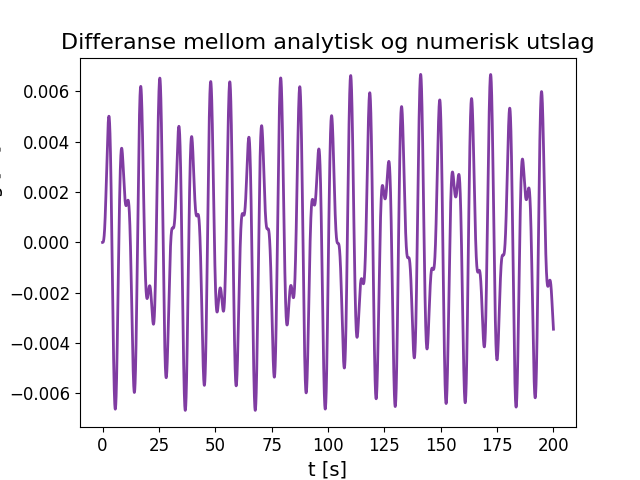
\includegraphics[scale=0.5]{Oppgave4_differanse.png}
\caption{viser differansen mellom den nummeriske og analytiske løsningen}
\label{fig:differanseplot}
\end{center}
\end{figure}

Så det nummeriske resultatet er ganske likt det analytiske. Plotter vi bevegelsen i faserommet får vi figur \ref{fig:faseplot4del1}

\begin{figure}[H]
\begin{center}
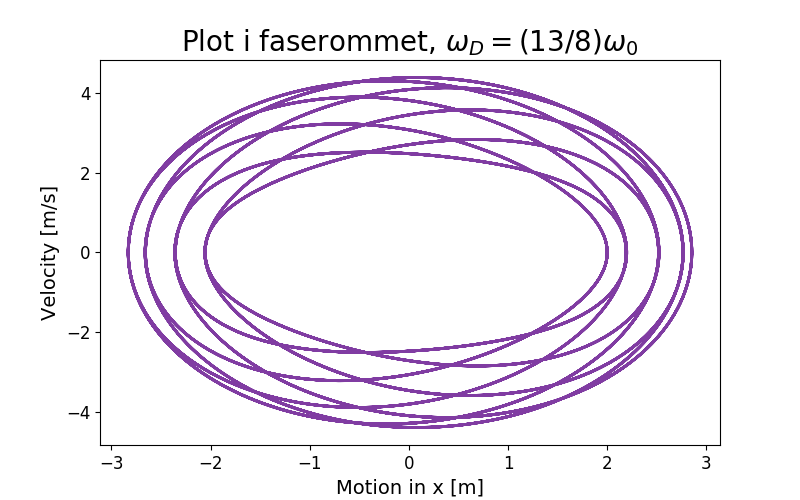
\includegraphics[scale=0.5]{Oppgave4fasedel1.png}
\caption{viser faseplottet med påtrykt kraft og $\omega_D = \frac{13}{8}\omega_0$}
\label{fig:faseplot4del1}
\end{center}
\end{figure}
Bevegelsen i figur \ref{fig:faseplot4del1} er periodisk. Hvis vi bytter ut drivefrekvensen med $\omega_D = \frac{2}{\left(\sqrt{5}-1 \right)}\omega_0$ så får vi 


\begin{figure}[H]
\begin{center}
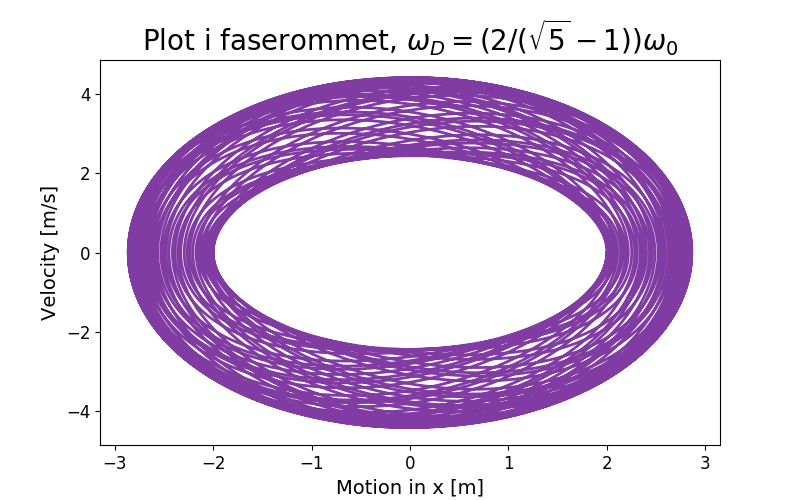
\includegraphics[scale=0.5]{Oppgave4fasedel2.png}
\caption{viser faseplottet med påtrykt kraft og $\omega_D = \frac{2}{\left(\sqrt{5}-1 \right)}\omega_0$}
\label{fig:faseplot4del2}
\end{center}
\end{figure}

Bevegelsen i figur \ref{fig:faseplot4del2} også en pariodisk bevegelse.



\section*{Oppgave 5}

mer ting
\begin{figure}[H]
\begin{center}
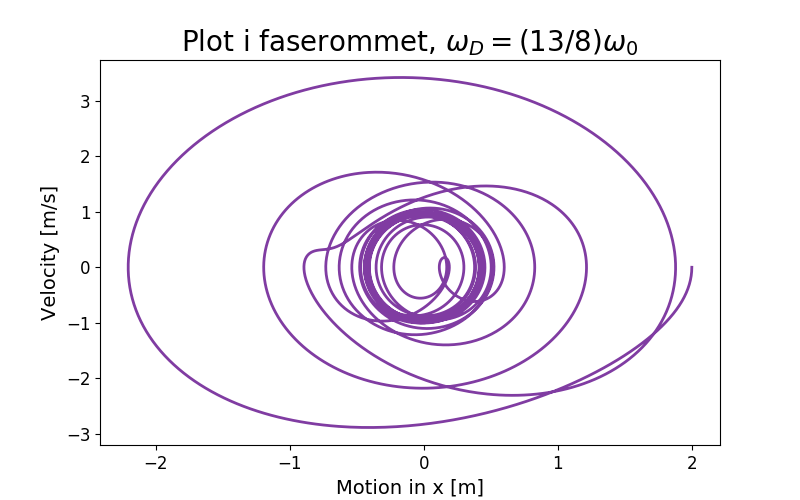
\includegraphics[scale=0.5]{Oppgave5fase1.png}
\caption{viser faseplottet med påtrykt kraft, dempning og $\omega_D = \frac{13}{8}\omega_0$}
\label{fig:faseplot5del1.png}
\end{center}
\end{figure}




\begin{figure}[H]
\begin{center}
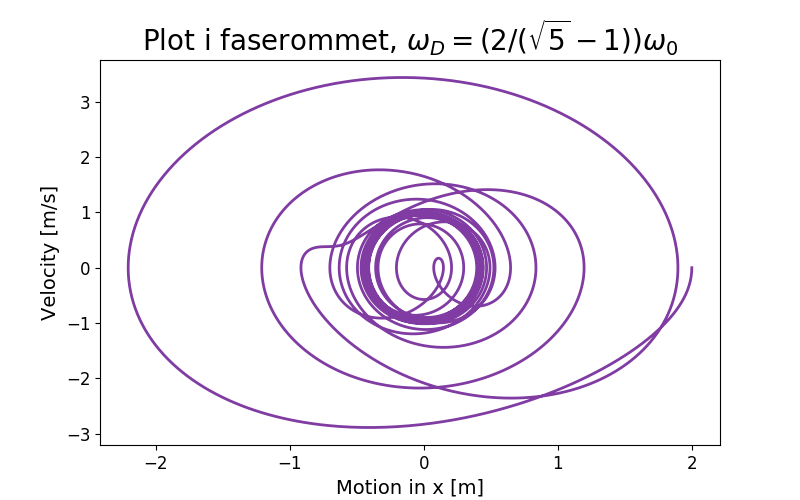
\includegraphics[scale=0.5]{Oppgave5fase2.png}
\caption{viser faseplottet med påtrykt kraft, dempning og $\omega_D = \frac{2}{\left(\sqrt{5}-1 \right)}\omega_0$}
\label{fig:faseplot5del2.png}
\end{center}
\end{figure}

Vi ser helt klart at banene i figur \ref{fig:faseplot5del1} og  \ref{fig:faseplot5del2} begynner likt som dere tilsvarende fra oppgave 4 og 2 men at de blir kaotiske fort og ender i en attraktor.

\section*{Oppgave 6}

\begin{figure}[H]
\begin{center}
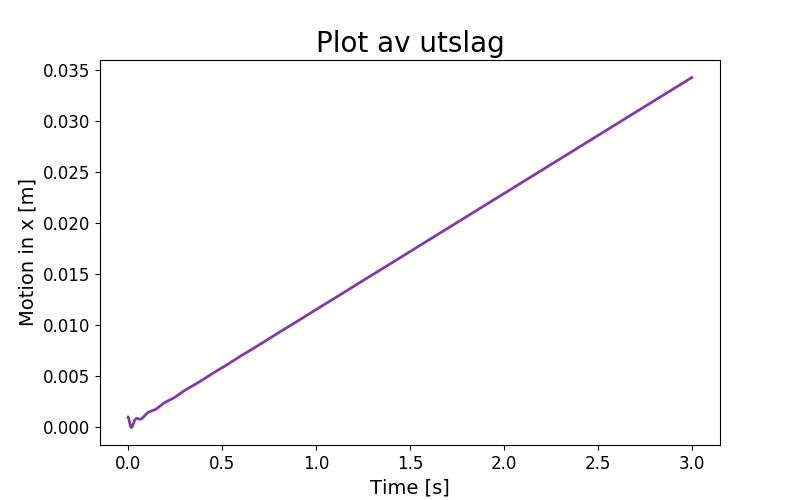
\includegraphics[scale=0.5]{Oppgave6utslag.png}
%\caption{viser faseplottet med påtrykt kraft, dempning og $\omega_D = \frac{2}{\left(\sqrt{5}-1 \right)}\omega_0$}
\label{fig:faseplot5del2.png}
\end{center}
\end{figure}

Posisjonen de første 3 sekundene øker gradvis. det ser realistisk ut fø dråpen faller.


\section*{Oppgave 7}

\begin{figure}[H]
\begin{center}
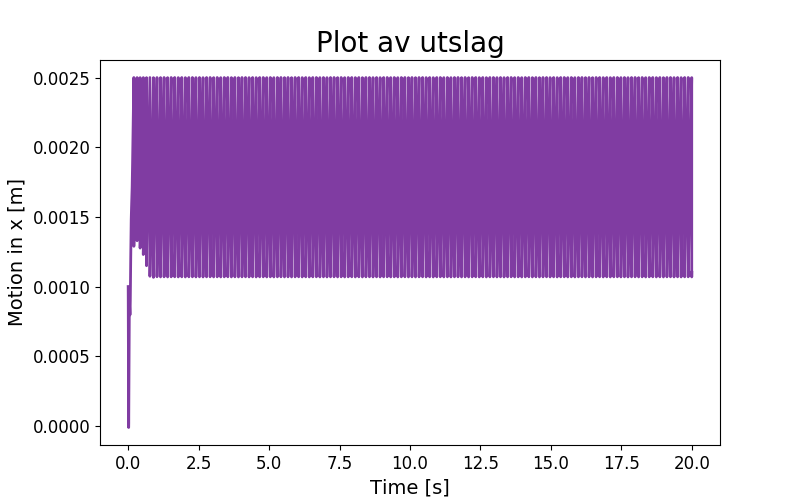
\includegraphics[scale=0.5]{Oppgave7utslag.png}
%\caption{viser faseplottet med påtrykt kraft, dempning og $\omega_D = \frac{2}{\left(\sqrt{5}-1 \right)}\omega_0$}
\label{fig:faseplot5del2.png}
\end{center}
\end{figure}


\begin{figure}[H]
\begin{center}
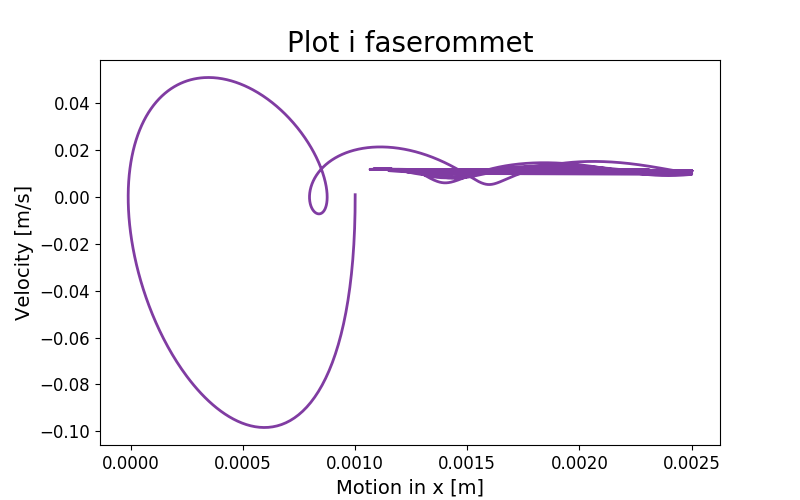
\includegraphics[scale=0.5]{Oppgave7faseplott.png}
%\caption{viser faseplottet med påtrykt kraft, dempning og $\omega_D = \frac{2}{\left(\sqrt{5}-1 \right)}\omega_0$}
\label{fig:faseplot5del2.png}
\end{center}
\end{figure}

Tiden mellom dråpene er konstant.


\section*{Oppgave 8}


Det blir et kjent form på plottet.


\section*{Oppgave 9}

Det jeg har fått likner på noe som ble funnet i andre artikler


\newpage


\section*{Appendix}

\lstinputlisting{RK4.py}

\lstinputlisting{oppgave1.py}

\lstinputlisting{oppgave2.py}

\lstinputlisting{oppgave4.py}

\lstinputlisting{oppgave5.py}

\lstinputlisting{oppgave6.py}

\lstinputlisting{oppgave7.py}

\lstinputlisting{oppgave8.py}


\end{document}